\chapter{METHODOLOGY}
\label{sec:chap3_metodologi}

\section*{ }
\section{Overview of the Icar System} 
The navigation system in Icar is divided into two types: the legacy navigation system using GNSS and the new navigation system that operates without GNSS. Below are block diagrams of Icar's navigation systems with and without GNSS.

\begin{figure}[H]
	\centering
	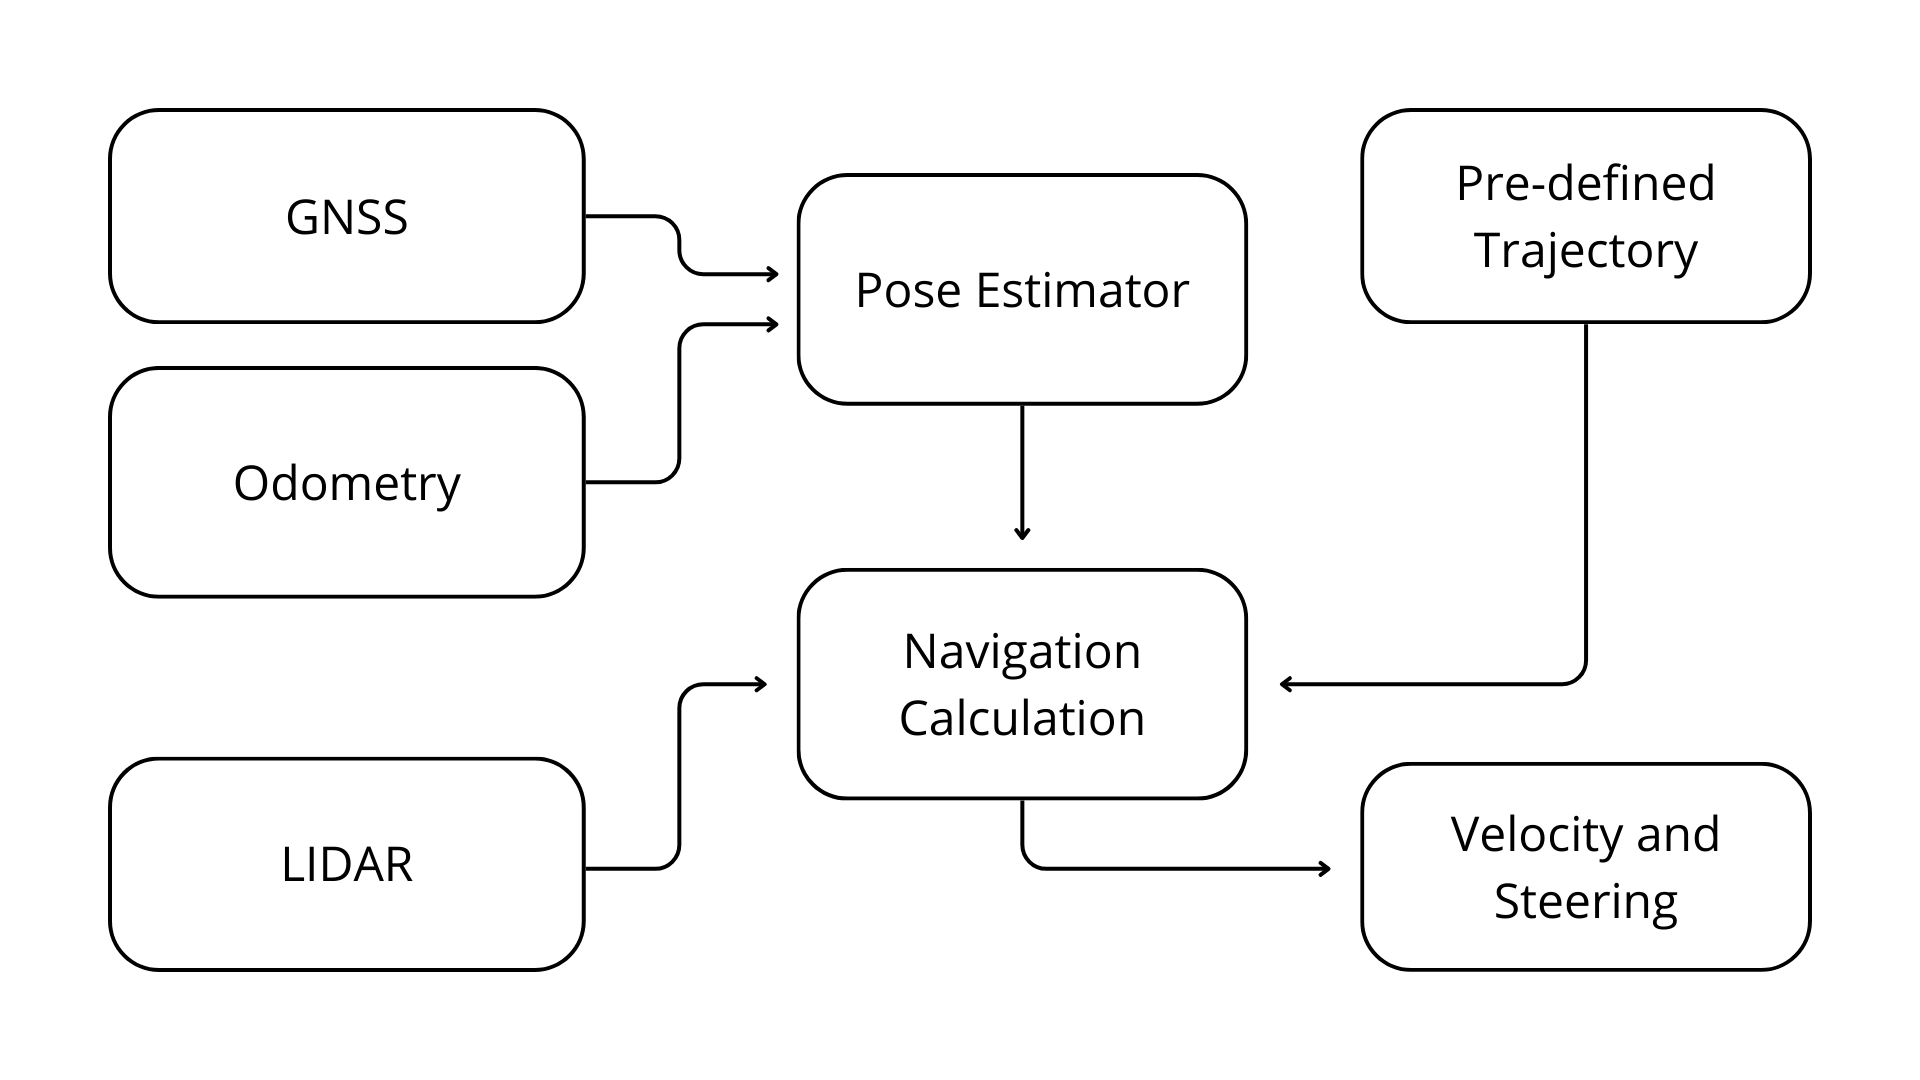
\includegraphics[width=\linewidth]{../konten/full_sys1.png}
	\caption{Block Diagram of the Legacy Icar System with GNSS}
	\label{fig:full_system}
\end{figure}
\FloatBarrier

Figure \ref{fig:full_system} illustrates the legacy Icar system, which relies on GNSS and odometry for pose estimation. The system uses a Pre-defined Trajectory to determine the target speed and steering angle using the Bicycle Model, as shown in equation~\ref{eq:bicycle_model_core}.

\begin{figure}[H]
	\centering
	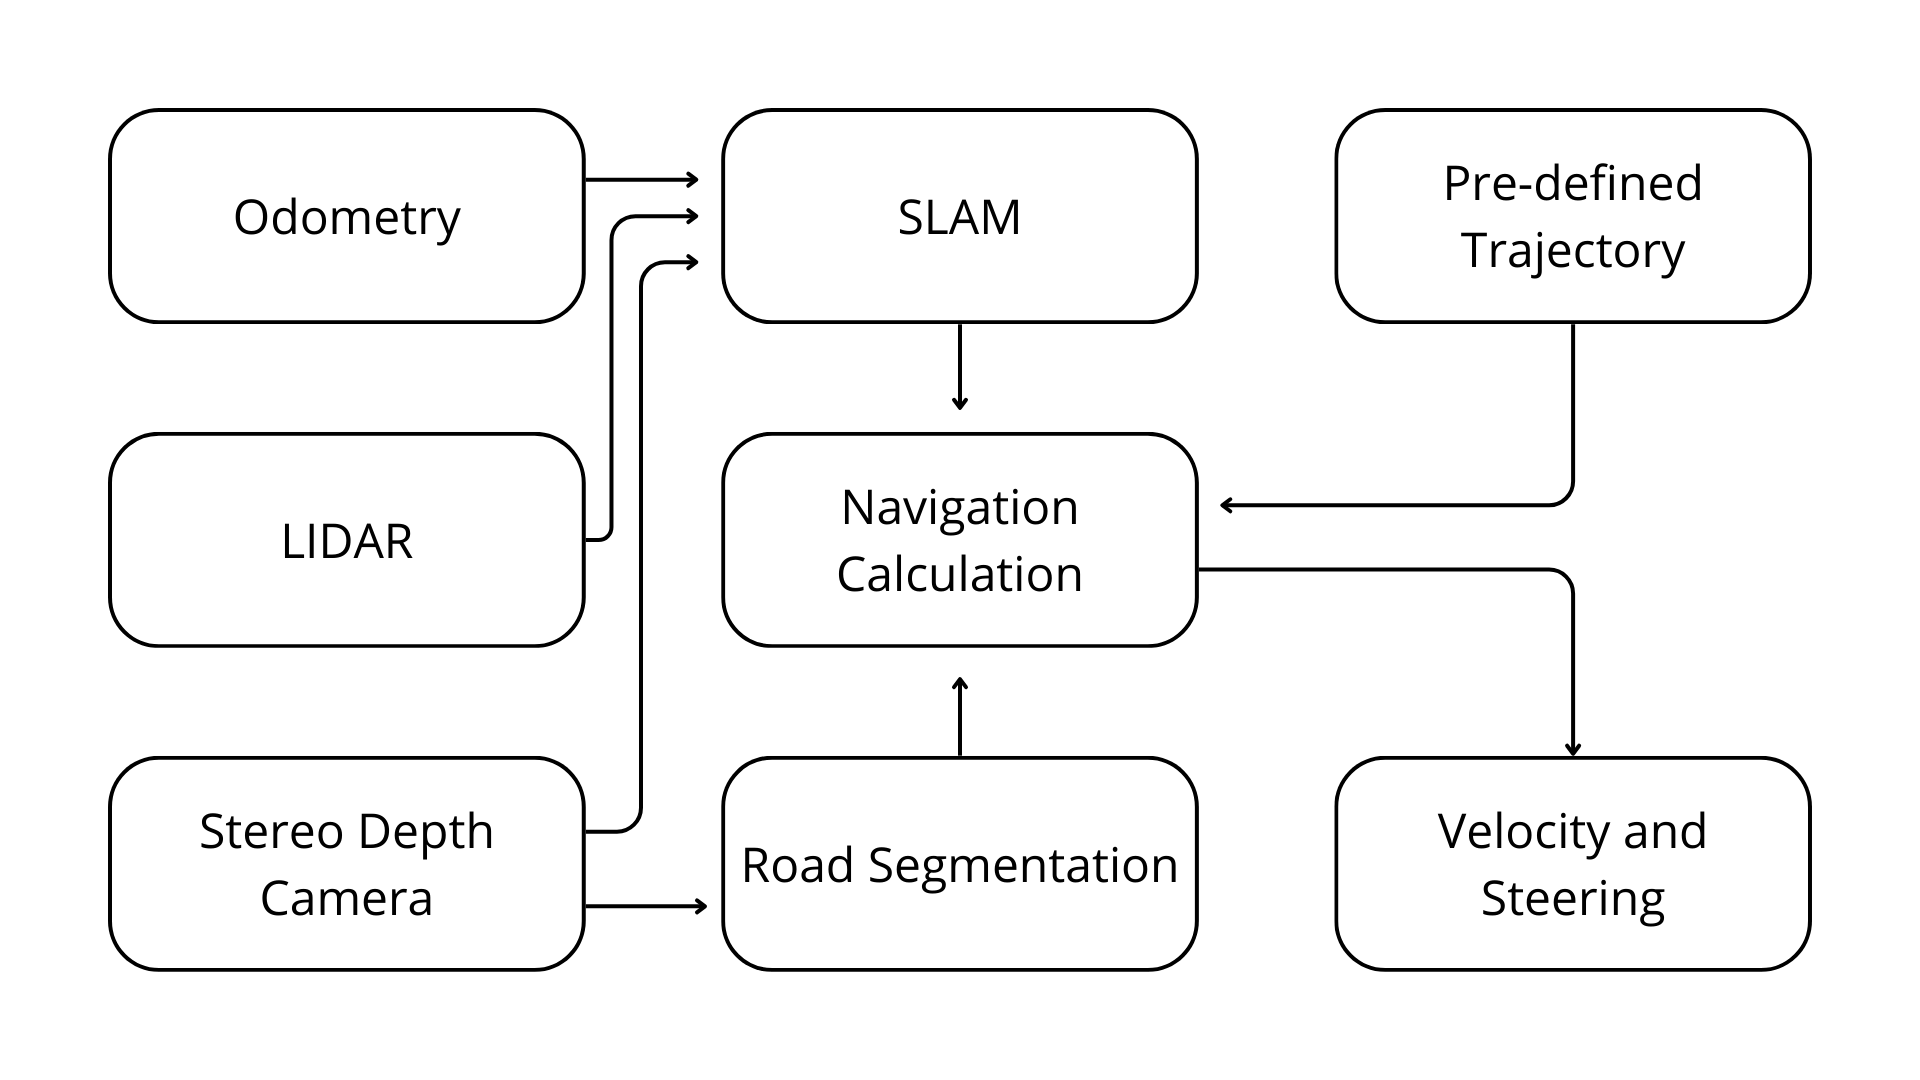
\includegraphics[width=\linewidth]{../konten/full_sys_slam1.png}
	\caption{Block Diagram of the New Icar System without GNSS}
	\label{fig:full_system_slam}
\end{figure}

Figure \ref{fig:full_system_slam} illustrates the new proposed Icar system, which does not rely on GNSS. Instead, it uses a stereo depth camera and LIDAR for pose estimation. The system also employs a Pre-defined Trajectory to determine the target speed and steering angle using the Bicycle Model \cite{rajamani2011vehicle}, as shown in equation \ref{eq:bicycle_model_core}. The first step is finding the target waypoint angle using equation below.
\begin{equation}
	\begin{aligned}
	\theta_{\text{direction}} = \tan^{-1}\left(\frac{y_{\text{waypoint}} - y_{\text{position}}}{x_{\text{waypoint}} - x_{\text{position}}}\right) - \theta_{\text{orientation}}
	\label{eq:waypoint_angle}
	\end{aligned}
\end{equation}
Where $x_{\text{waypoint}}$ and $y_{\text{waypoint}}$ are the coordinates of the waypoint obtained from the Pre-defined Trajectory, $x_{\text{position}}$ and $y_{\text{position}}$ represent the vehicle's current position, and $\theta_{\text{orientation}}$ is the current orientation of the vehicle. $\theta_{\text{direction}}$ is the heading angle towards the waypoint. With using that angle, we can calculate the target steering angle by using the Bicycle Model as follows:

\begin{equation}
	\begin{aligned}
	\delta_{\text{target}} = \tan^{-1}\left( \frac{2 \cdot L \cdot \sin(\theta_{\text{direction}})}{D_{\text{lookahead}}} \right)
	\label{eq:bicycle_model_full}
	\end{aligned}
\end{equation}
Where $L$ is the distance between the front and rear wheels, and $D_{\text{lookahead}}$ is the lookahead distance. $\delta_{\text{target}}$ is the target steering angle. The target speed is calculated using the following equation:

\begin{equation}
	\begin{aligned}
		v_{\text{target}} &= \min\left(\sqrt{(y_{\text{waypoint}} - y_{\text{position}})^2 + (y_{\text{waypoint}} - y_{\text{position}})^2}, \ v_{\text{max}}\right) \\
		\label{eq:bicycle_model_velocity}
	\end{aligned}		
\end{equation}
Where $v_{\text{max}}$ is the maximum speed of the vehicle. The target speed $v_{\text{target}}$ is determined by the distance to the waypoint, ensuring it does not exceed the maximum speed.

The primary difference between the two systems is the source of position and orientation data. The legacy system uses GNSS and odometry, while the new system uses stereo depth cameras, LIDAR, and odometry. Additionally, the new system integrates road detection to enhance navigation safety.

\section{Road Detection System}
\begin{figure}[H]
	\centering
	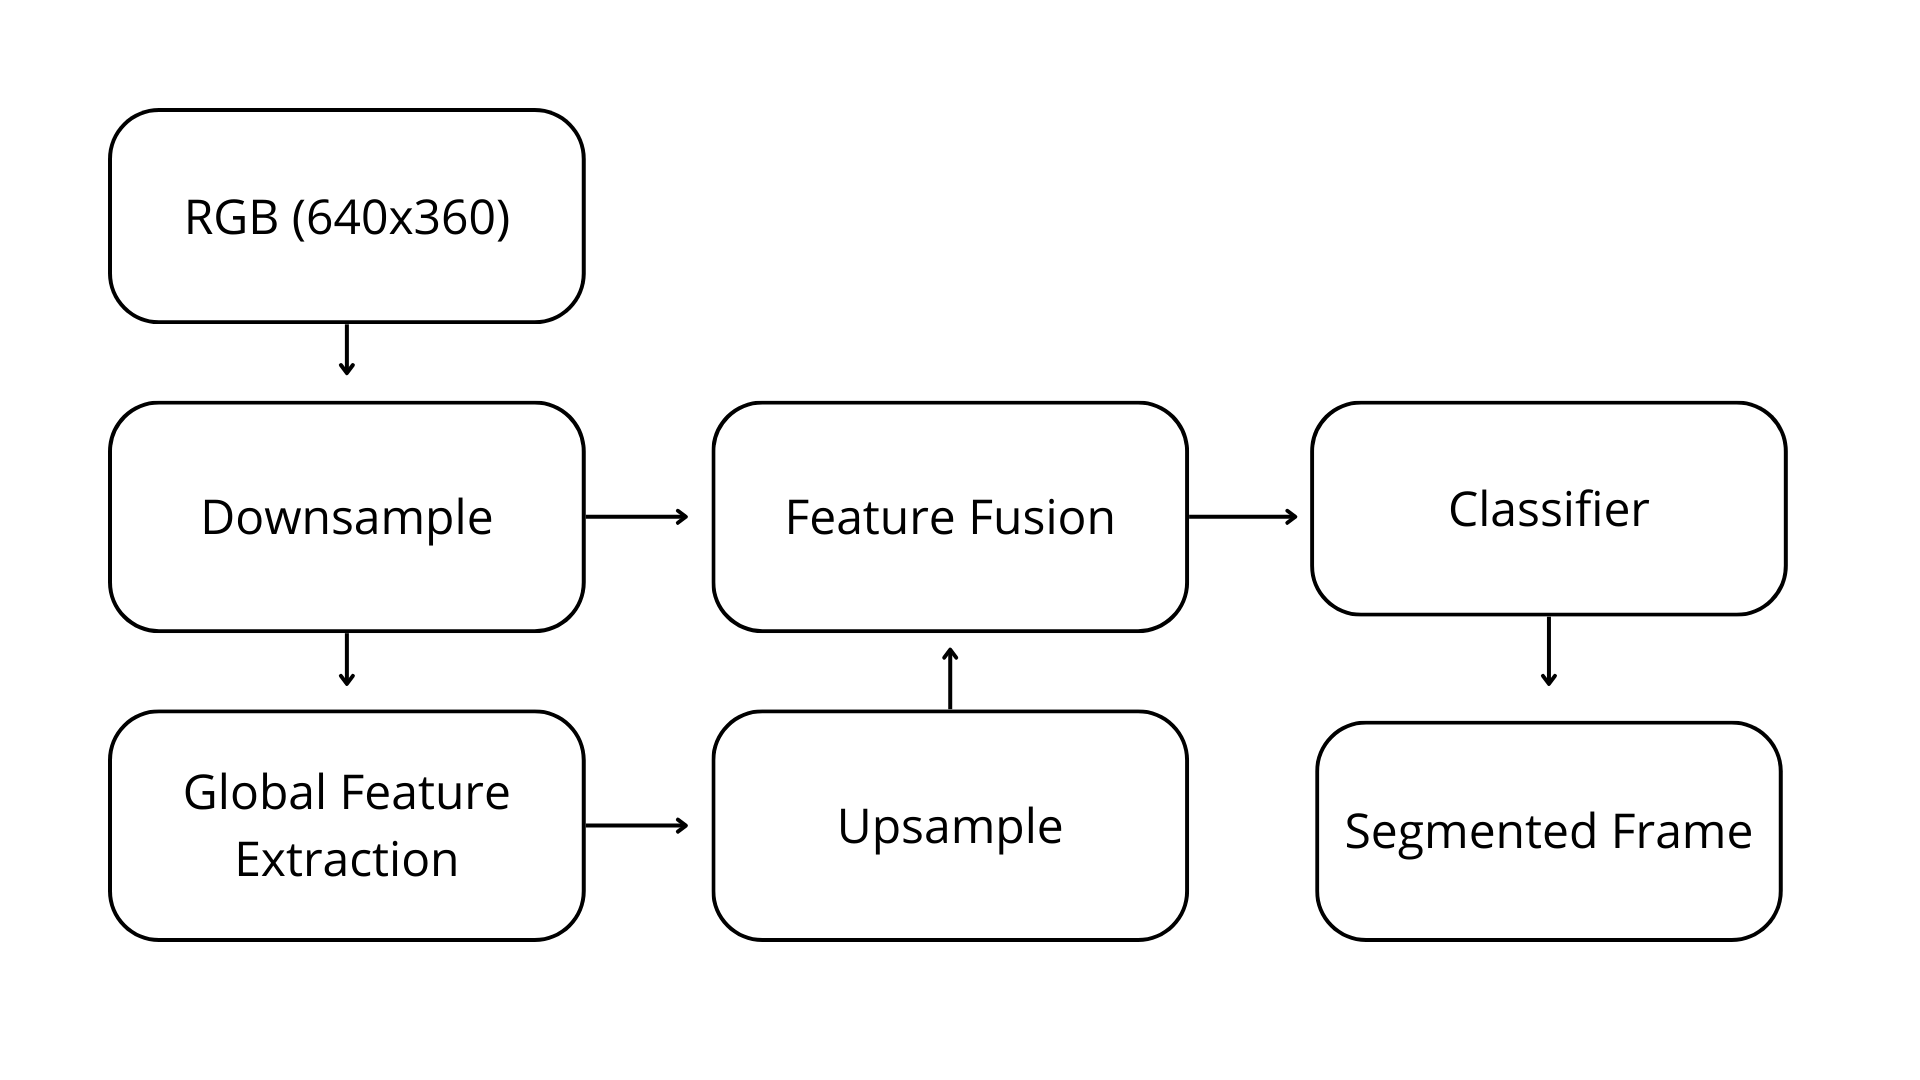
\includegraphics[width=\linewidth]{../konten/ml_sys.png}
	\caption{Block Diagram of the Machine Learning Architecture on Icar}
	\label{fig:ml_system}
\end{figure} 

From Figure \ref{fig:ml_system}, it is shown that the road detection system on Icar utilizes a machine learning architecture, specifically using Fast-SCNN \cite{ref_fast_scnn} as the core model. Its architecture differs in the convolution channels and pooling methods. The smaller convolution channels and the use of average pooling instead of pyramid pooling are intended to reduce computational load, making it suitable for real-time applications on Icar.

\subsection{Downsampling} 
Figure \ref{fig:ml_capture} shows the raw image captured by the stereo depth camera. The image is then processed through a series of convolution layers to downsample it.
\begin{figure}[H]
	\centering
	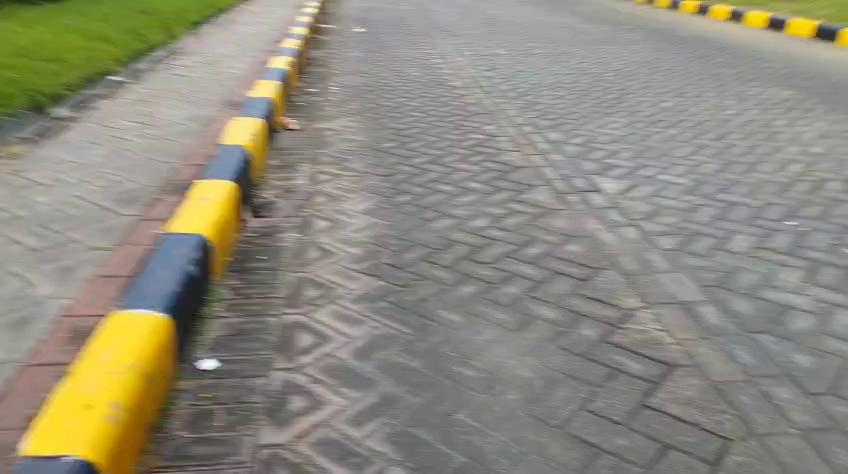
\includegraphics[width=\linewidth]{../konten/asli.png}
	\caption{Raw Image}
	\label{fig:ml_capture}
\end{figure} 
In this step, the image captured by the stereo depth camera, originally a 3-channel image, is converted to 16 channels. This is achieved via three successive 3x3 convolution layers with a stride of 2: first converting 3→8 channels, then 8→16, and finally 16→32 channels. The resulting image is then split into two paths: one goes to global feature extraction, the other to feature fusion. 
\begin{figure}[H]
	\centering
	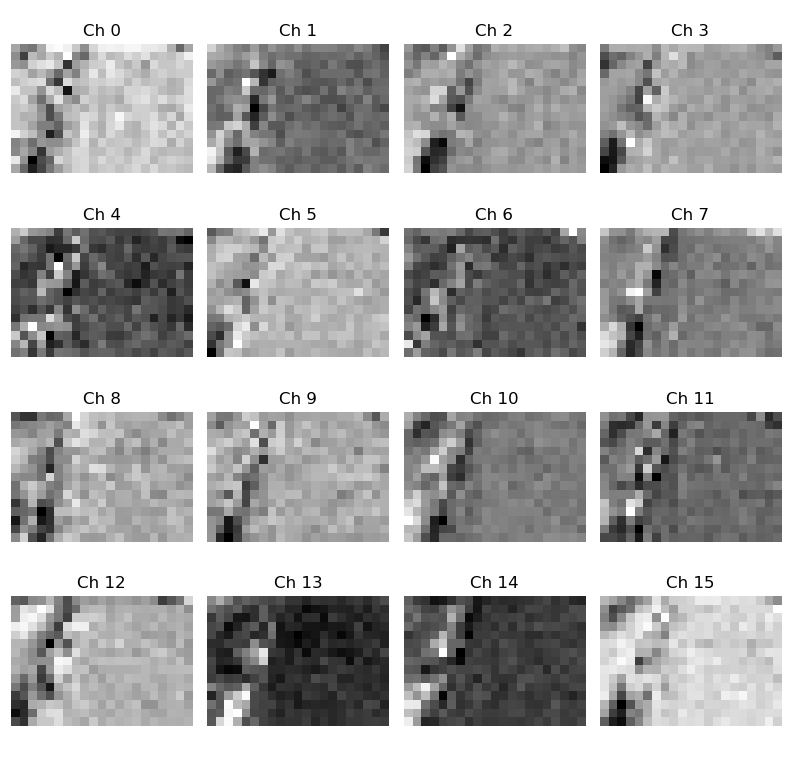
\includegraphics[width=\linewidth]{../konten/ds_b3.png}
	\caption{Result of Downsampling Stage}
	\label{fig:ml_ds}
\end{figure} 
Figure \ref{fig:ml_ds} shows the result of the downsampling stage, where the original 3-channel image is transformed into a 32-channel image (but the figure only shows 16 channel because it was too much to show all 32 channels). This image is then processed further in the global feature extraction and upsampling stages.

\subsection{Global Feature Extraction}
This stage performs a depthwise-separable convolution to extract features from the 32-channel image. This method is chosen for its computational efficiency. The result is a 48-channel image, which is passed on to the upsampling stage. 
\begin{figure}[H]
	\centering
	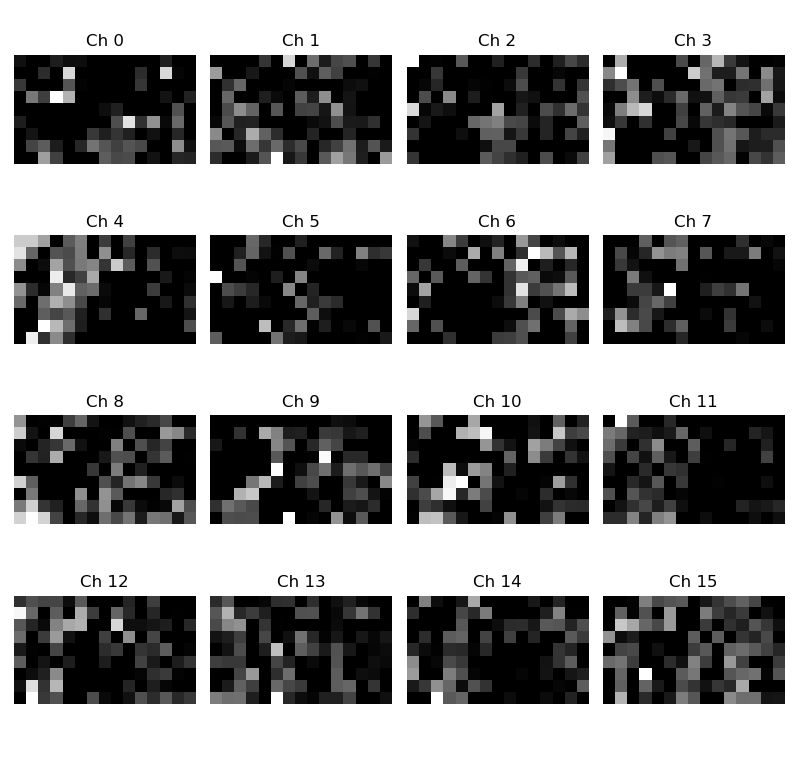
\includegraphics[width=\linewidth]{../konten/gf_0.png}
	\caption{Result of Feature Extraction Stage}
	\label{fig:ml_gf}
\end{figure} 
Figure \ref{fig:ml_gf} shows the result of the global feature extraction stage, where the 32-channel image is processed to produce a 48-channel image. This image contains the extracted features that will be used in the subsequent upsampling and feature fusion stages.

\subsection{Upsampling}
This step performs pooling using average pooling, which is lighter and faster compared to the pyramid pooling used in the original Fast-SCNN. A convolution then produces a 64-channel output, which is passed to feature fusion.
\begin{figure}[H]
	\centering
	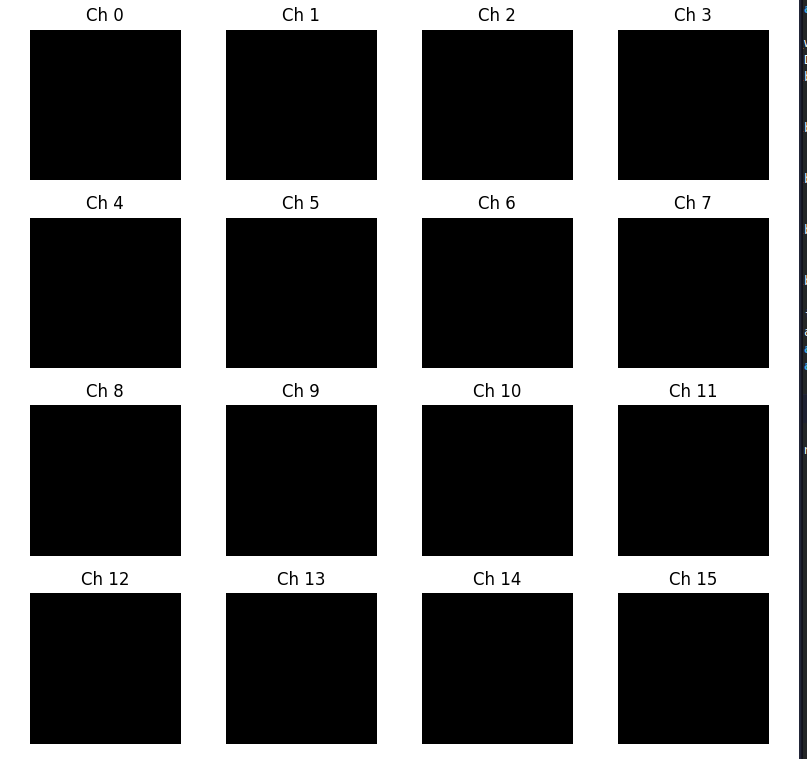
\includegraphics[width=\linewidth]{../konten/gf_1.png}
	\caption{Result of Upsampling Stage}
	\label{fig:ml_gf1}
\end{figure} 
Figure \ref{fig:ml_ds} shows the result of the upsampling stage, where the 48-channel image from the global feature extraction stage is processed to produce a 64-channel image. This image is then ready for merging with the downsampled features in the feature fusion stage.

\subsection{Feature Fusion}
Here, outputs from the downsampling (32 channel) and global feature extraction (64 channel) stages are merged into a 96-channel image. Before merging, image dimensions are matched using bilinear interpolation. The merged result is passed to the classification stage.

\subsection{Classification}
In this final stage, the 96-channel image undergoes classification using ReLU, producing a 1-channel image indicating road areas. This image then proceeds to post processing.
\begin{figure}[H]
	\centering
	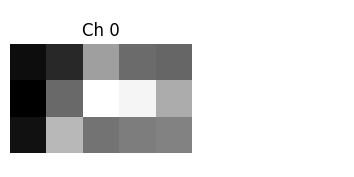
\includegraphics[width=6cm]{../konten/class_1.png}
	\caption{Result of Classification Stage}
	\label{fig:ml_cls0}
\end{figure} 
Figure \ref{fig:ml_cls0} shows the result of the classification stage, where the 96-channel image from the feature fusion stage is processed to produce a 1-channel image. 

\section{Pose and Orientation Correction System}
\begin{figure}[H]
	\centering
	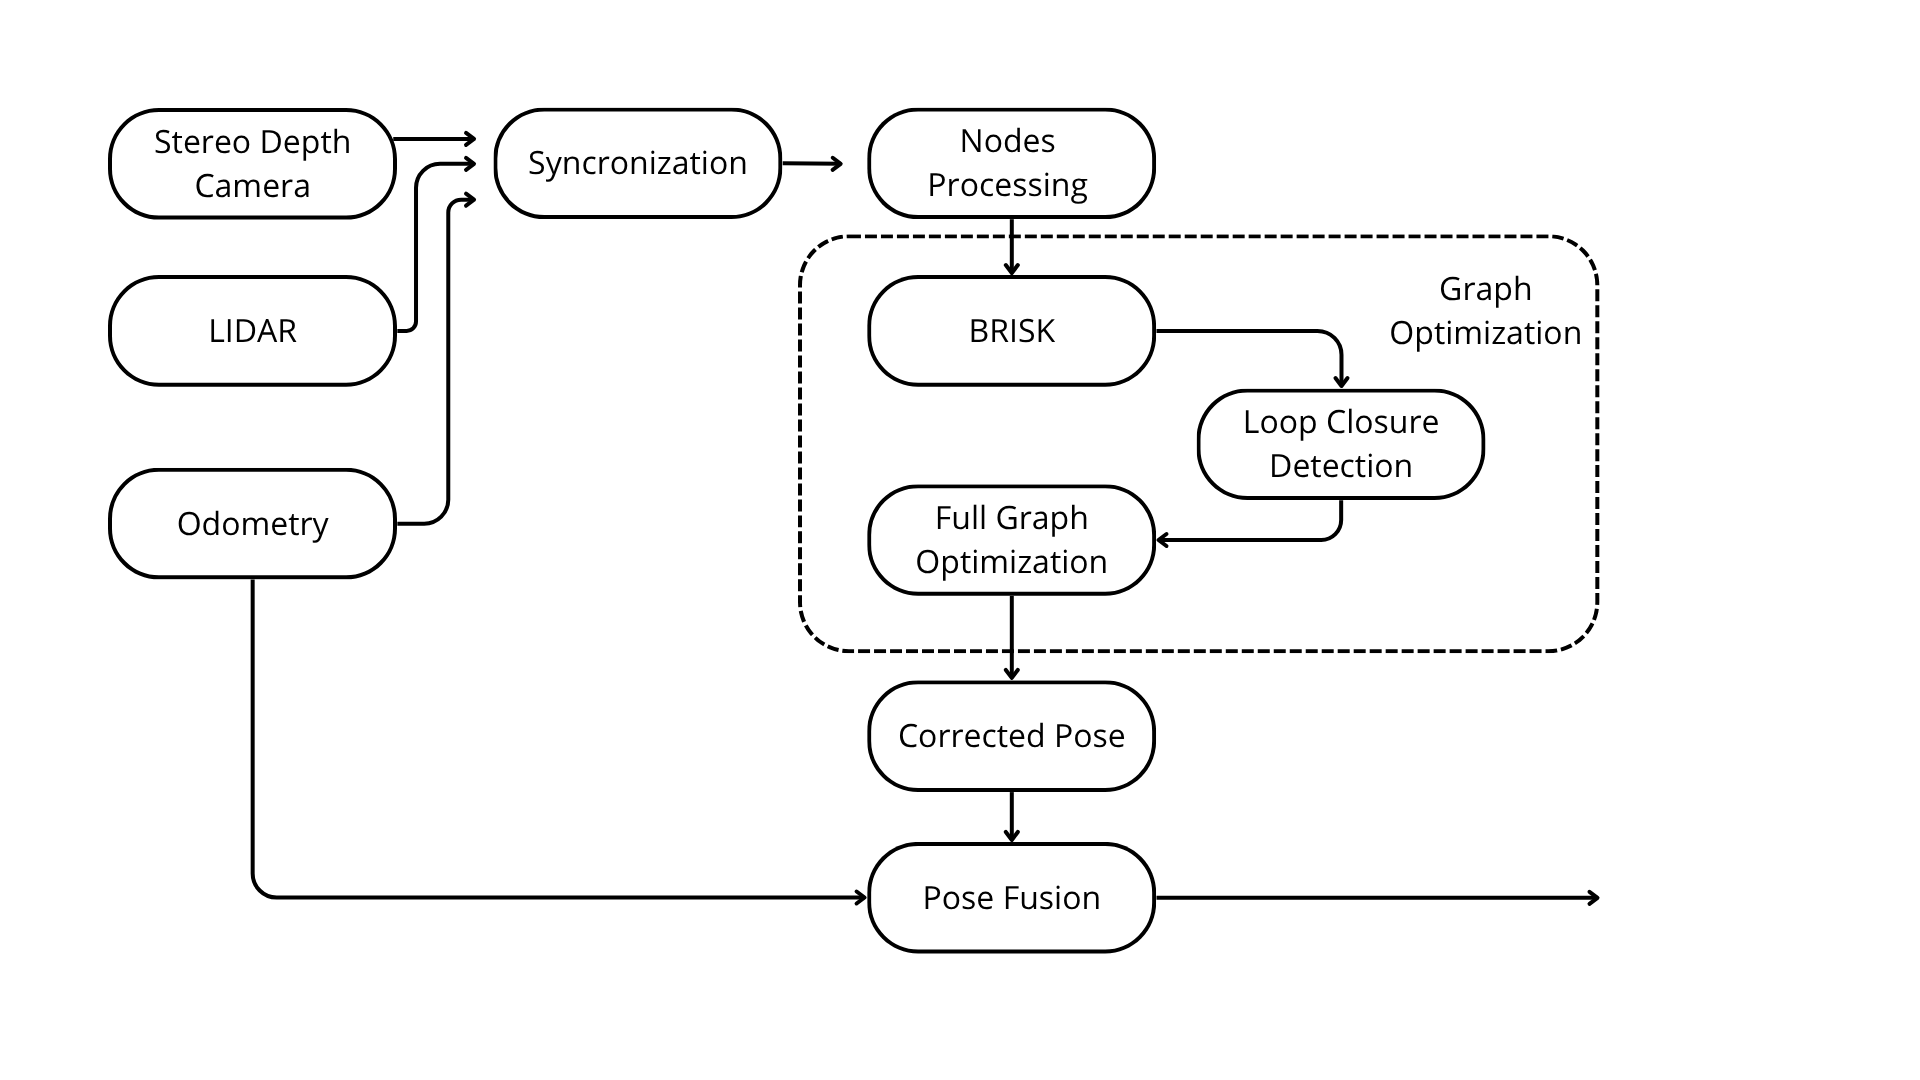
\includegraphics[width=\linewidth]{../konten/GNSS(20).png}
	\caption{Block Diagram of Pose and Orientation Correction System on Icar}
	\label{fig:slam_system}
\end{figure} 

From Figure \ref{fig:slam_system}, the pose correction system consists of four main processes: data synchronization, nodes processing, graph optimization, and pose fusion.

\subsection{Data Synchronization} 
This initial step synchronizes data from the stereo depth camera and odometry based on timestamps to ensure aligned data for further processing. The technique that used is the approximate time synchronization. Approximate time synchronization assume that the error timestamp below threshold like 10 milliseconds is eligible to be synchronized. 

\subsection{Nodes Processing}
This initiates the graph optimization process. Nodes represent vehicle poses and keypoints from stereo depth camera and LIDAR. There are two modes in this process, the first mode is mapping mode. In mapping mode, the system creates new nodes for each pose, keypoint detected by the stereo depth camera and LIDAR laser scan while the robot has moved 1 meter away from the last node created. The second mode is localization mode, where existing nodes are used without adding new ones. This mode is used when the vehicle is already in a known area, and it needs to localize itself within that area without creating new nodes. Mapping mode only used once, while localization mode is used every time the vehicle is moving after finished mapping mode.

\subsection{Graph Optimization} 
The first step is finding the loop closure by using BRISK algorithm \cite{ref_brisk}. BRISK will doing image matching between the current image and the previous saved image for each node. If the image matches, it will be considered as loop closure hypothesis. Then by using GTSAM \cite{ref_gtsam}, the optimization error will be calculated for all nodes by doing ICP \cite{ref_icp} from the saved LIDAR laser scan for each node. If the optimization error less than the threshold (3.0), the loop closure will be accepted, and the graph will be optimized. The optimization process uses a factor graph approach, where each node represents a pose and each edge represents a constraint between poses. The optimization minimizes the error in pose estimation by adjusting the poses based on the constraints.

\subsection{Pose Fusion} 
The final step combines poses from graph optimization and odometry using a Kalman Filter, resulting in more accurate pose estimation than using odometry alone. Using the differential data from Odometry (Wheel encoder and IMU) combined with estimated pose that coming from Graph Optimization, the system can correct the pose and orientation of Icar. 

\section{Icar Navigation System with Road Detection and Graph-Based SLAM} 
\begin{figure}[H]
	\centering
	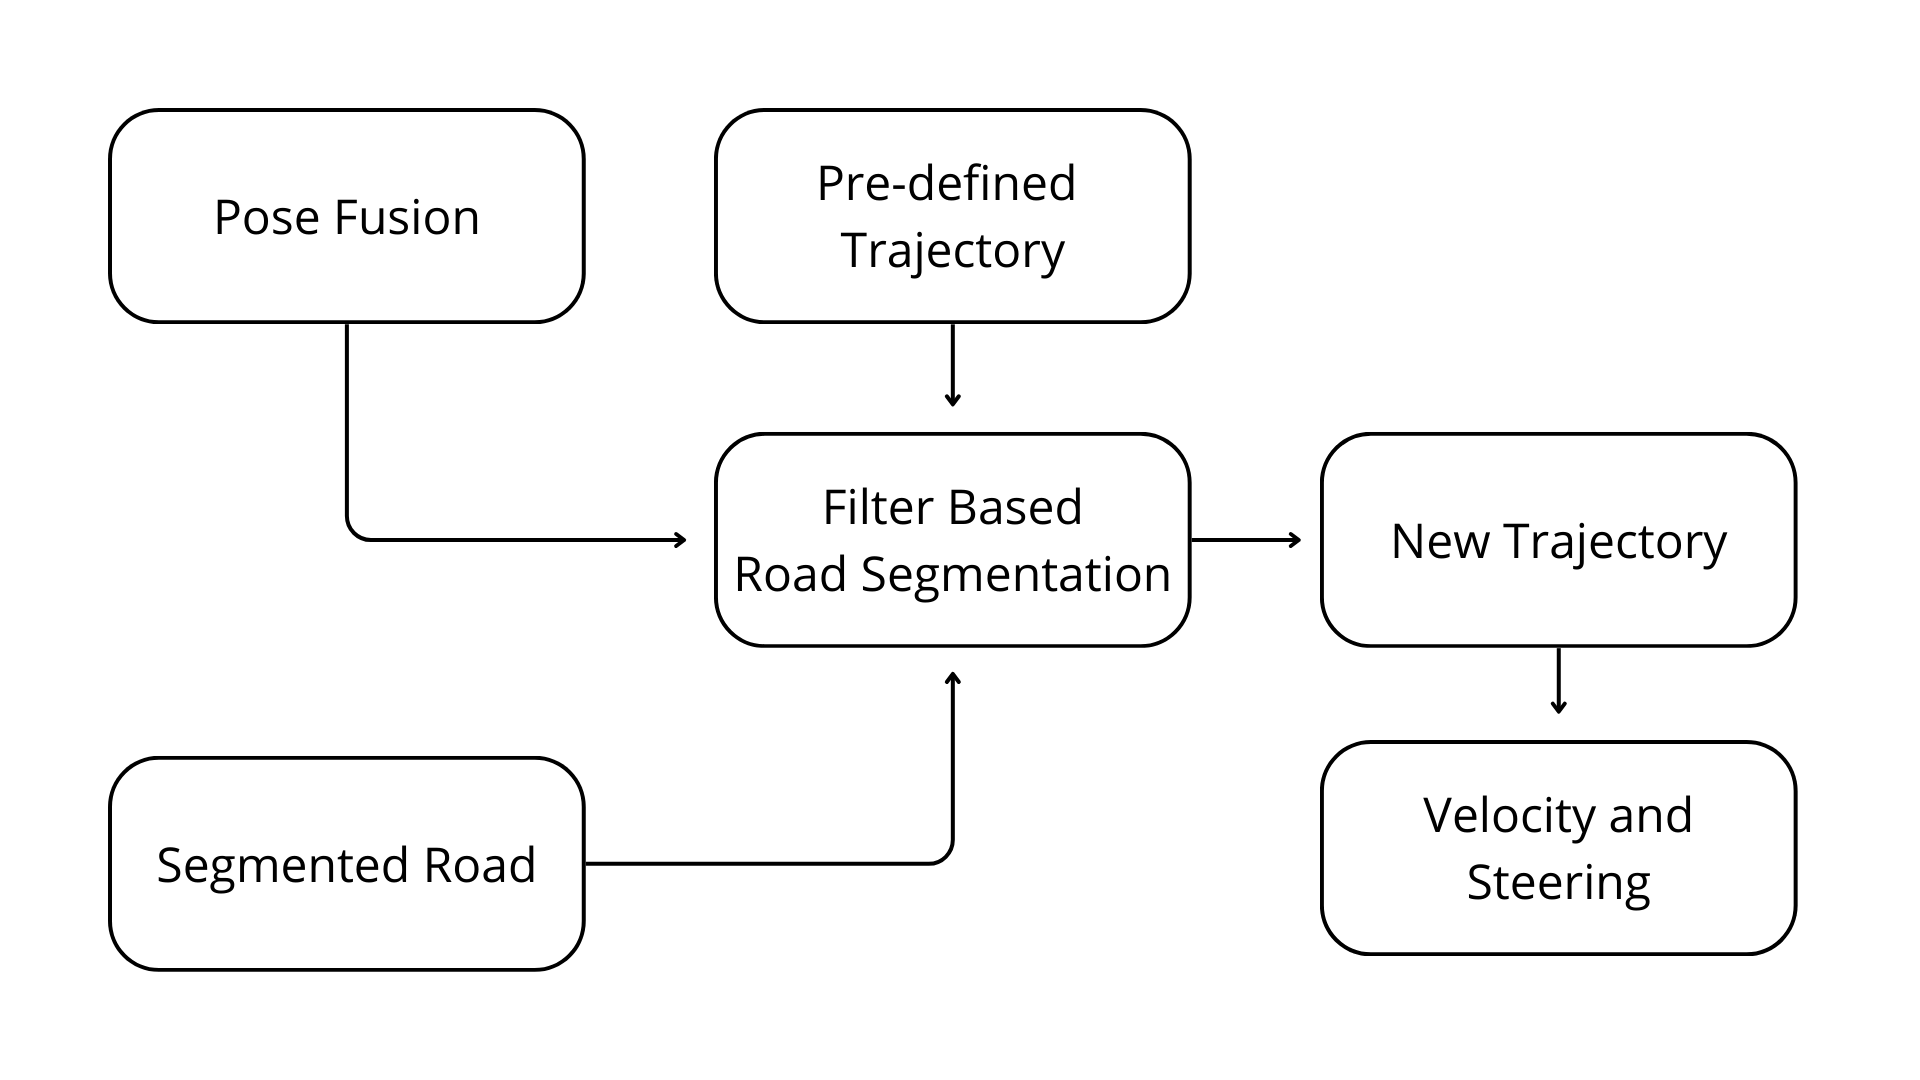
\includegraphics[width=\linewidth]{../konten/nav_new_sys3.png}
	\caption{Block Diagram of Icar Navigation System with Road Detection and Graph-Based SLAM}
	\label{fig:nav_new_system}
\end{figure} 

This diagram expands upon Figure \ref{fig:full_system_slam}, showing how the segmented road image from Figure \ref{fig:ml_system} and the pose data from Figure \ref{fig:slam_system} are integrated into a unified and improved navigation system.

\par  
The first step selects waypoints based on current pose (from graph-based SLAM) and the pre-defined trajectory. These waypoints are overlaid on the road segmentation image.

\par   
Next, a check is performed using a bitwise AND operation to determine if all waypoints lie within the road area. If so, the selected waypoints are used as the new trajectory.

\par  
If any waypoint lies outside the road, a new trajectory is generated using the image’s center of mass, converted into vehicle coordinates. A straight line is then created from the current position to the center of mass.

\begin{figure}[H]
	\centering
	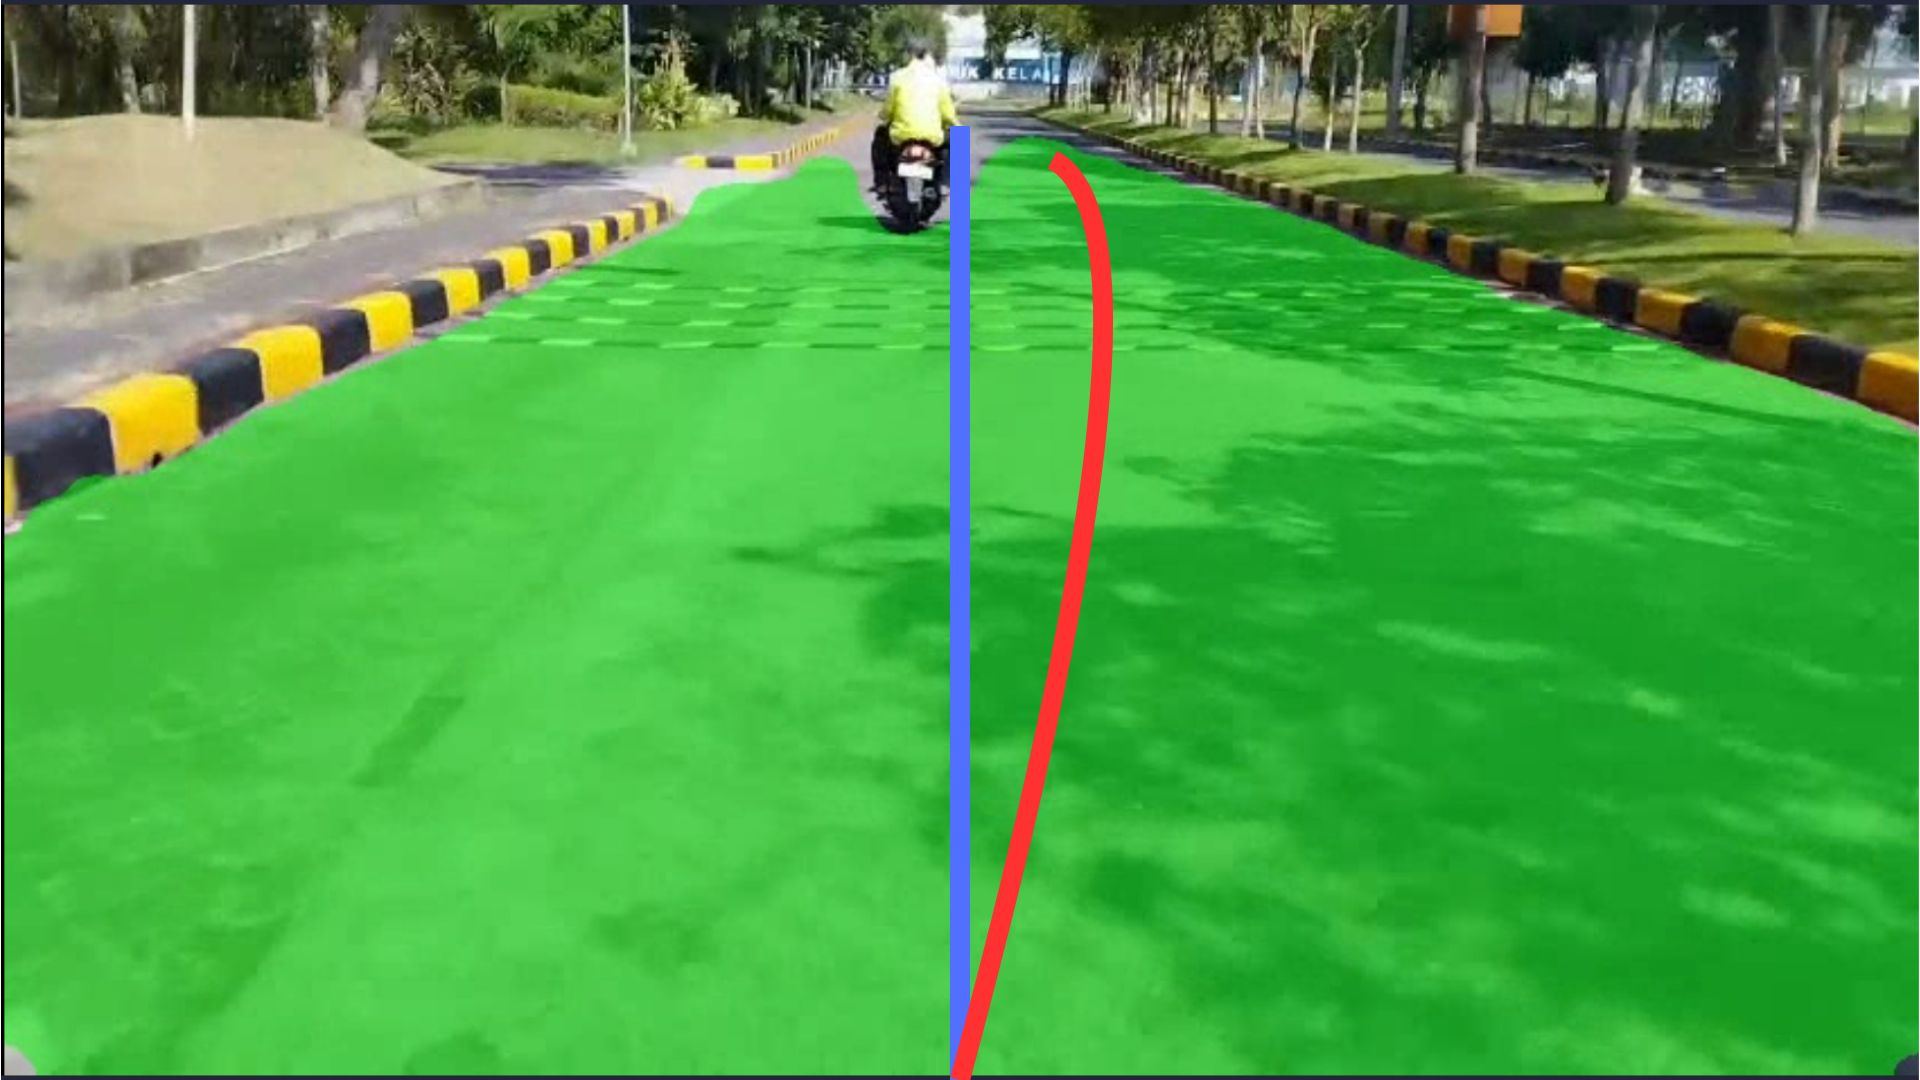
\includegraphics[width=\linewidth]{../konten/contoh_hasil_edited.png}
	\caption{Visualization of the Road Detection and Graph-Based SLAM Results on Icar}
	\label{fig:nav_visualize_contoh}
\end{figure} 
Where the green mask is the segmented road, the blue line is the trajectory that coming from the pre-defined trajectory, the red line is the new trajectory that generated from this research. The vehicle will follow the red line as the new trajectory. 

\par 
This new trajectory is then used for vehicle navigation. The vehicle follows it using the Bicycle Model as defined in Equation \ref{eq:bicycle_model_full} and \ref{eq:bicycle_model_velocity} to calculate target speed and steering angle.
